\section{Legge di Snell e reversibilità del cammino ottico}
La velocità di propagazione della luce è costante nel vuoto, ma diminuisce se attraversa un mezzo. Ogni materiale è caratterizzato da un indice di rifrazione, dato dal rapporto fra velocità della luce nel vuoto e nel mezzo \[n=\frac{c}{v}\] Esso è sempre maggiore di 1 e dipende dalla lunghezza d'onda della luce. Quando un raggio luminoso attraversa la superficie di separazione fra due mezzi diversi, avviene un fenomeno detto rifrazione. La relazione tra l'angolo di incidenza e l'angolo di rifrazione è descritta dalla legge di Snell 

\begin{equation}
    n_1 \sin{\theta_{\text{incidente}}} = n_2 \sin{\theta_{\text{rifratto}}}
    \label{Legge di Snell}
\end{equation}

dove $n_1$ e $n_2$ sono i rispettivi indici di rifrazione, mentre $\theta_{\text{rifratto}}$ e $\theta_{\text{incidente}}$ sono gli angoli misurati rispetto alla normale alla superificie come mostrato in figura.

\begin{figure}[htbp]
    \centering
    \begin{tikzpicture}[scale=1.5] % Scala il disegno se lo vuoi più grande o piccolo
        
        % 1. Definizione dei colori e dello sfondo (Acqua/Vetro in basso)
        \fill[blue!10] (-3,-2) rectangle (3,0);
        \node[anchor=north west] at (-3,-1.5) {Mezzo 2 ($n_2 > n_1$)};
        \node[anchor=south west] at (-3,1.5) {Mezzo 1 ($n_1$)};
        
        % 2. Interfaccia di separazione e retta Normale
        % CORRETTO: font=\small inserito nelle opzioni del nodo
        \draw[thick] (-3,0) -- (3,0); 
        \node[anchor=north] at (2.5,0.5) [font=\small] {Superficie di separazione};
        \draw[dashed] (0,-2) -- (0,2) node[above] {Normale};
        
        % 3. Definizione dei punti chiave per gli angoli
        \coordinate (O) at (0,0);     % Punto di incidenza (origine)
        \coordinate (N_top) at (0,2); % Punto in alto sulla normale
        \coordinate (N_bot) at (0,-2);% Punto in basso sulla normale
        \coordinate (A) at (-1.5,1.5);% Origine del raggio incidente
        \coordinate (B) at (1,-1.73); % Fine del raggio rifratto
        
        % 5. Disegno degli angoli (i e r)
        % Angolo di incidenza
        \pic [draw, angle radius=1cm, angle eccentricity=1.6, fill=green!22] {angle = N_top--O--A};
        \node[anchor=south] at (0.7,0.6) [font=\small] {$\theta_{\text{\text{incidente}}}$};
        % Angolo di rifrazione

        \node[anchor=north] at (-0.5,-0.3) [font=\small] {$\theta_{\text{\text{rifratto}}}$};
        \pic [draw, angle radius=1cm, angle eccentricity=1.6, fill=yellow!22] {angle = N_bot--O--B};
        
        \draw[red, thick, ->] (A) -- (O) node[midway, left, font=\small] {Raggio Incidente};
        \draw[red, thick, ->] (O) -- (B) node[midway, right, font=\small] {Raggio Rifratto};
        
    \end{tikzpicture}
    \caption{Diagramma della rifrazione della luce con legge di Snell.}
    \label{fig:rifrazione}
\end{figure}

Inoltre, la legge di Snell prevede la reversibilità del cammino ottico. Se si fa incidere il raggio luminoso ad un angolo pari a $\theta_{\mathrm{\text{rifratto}}}$ si deve ottenere \(\theta'_{\mathrm{\text{rifratto}}}=\theta_{\mathrm{incidenza}}\).

Questa prima parte dell'esperimento è stata effettuata utilizzando una lente semicilindrica in plexiglass. Quando un raggio luminoso incide nel centro della faccia piana della lente subisce un'unica rifrazione all'ingresso. Infatti, poiché il raggio interseca la superficie curva lungo la normale nel passaggio dalla lente all'aria, non varia la sua traiettoria in uscita.
Le misure degli angoli di rifrazione sono state effettuate considerando come errore la precisione del goniometro presente sulla piattaforma, ovvero $\sigma_{\theta}=\ang{1}$. 
\newpage
Si riportano i dati raccolti in Tabella 1:\\

\begin{table}[H]
\centering    
\label{tab:angoli-rifrazione}
\small
\begin{tabular}{cc cc}
\toprule
\multicolumn{2}{c}{\textbf{Incidenza}} & \multicolumn{2}{c}{\textbf{Rifrazione}} \\
\cmidrule(r){1-2} \cmidrule(l){3-4}
$\theta_{\text{inc}}$ & $\sin\theta_{\text{inc}}$ & $\theta_{\text{rif}}$ & $\sin\theta_{\text{rif}}$ \\ 
\midrule
$20^{\circ}$ & 0.342 & $13^{\circ}$ & 0.225 \\
$25^{\circ}$ & 0.423 & $16^{\circ}$ & 0.276 \\
$30^{\circ}$ & 0.500 & $20^{\circ}$ & 0.342 \\
$45^{\circ}$ & 0.707 & $28^{\circ}$ & 0.469 \\
$60^{\circ}$ & 0.866 & $35^{\circ}$ & 0.574 \\
$70^{\circ}$ & 0.940 & $39^{\circ}$ & 0.629 \\
\bottomrule
\end{tabular}
\caption{Angoli di rifrazione per la lente semicilindrica.}
\end{table}

È stata effettuata un'interpolazione lineare passante per l'origine tra $\sin\theta_{\text{inc}}$ e $\sin\theta_{\text{rif}}$, dalla quale si ricava k=0.66 $\pm$ 0.01. Il test del $\chi^2$ restituisce un $\tilde{\chi_o}^2= 0.10$, che per 5 gradi di libertà corrisponde a una compatibilità coi dati del $99.3\%$.
Si riporta di seguito il grafico:
\begin{figure}[h!]
    \centering
    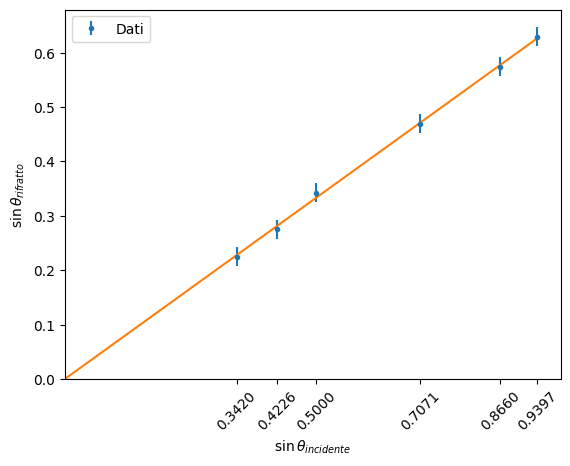
\includegraphics[width=0.8\textwidth]{immagini/Legge di Snell.png}
    \caption{Interpolazione lineare passante per l'origine tra $\sin\theta_{\text{inc}}$ e $\sin\theta_{\text{rif}}$.}
    \label{fig:mia_immagine}
\end{figure}

Dalla legge di Snell si ricava $k=\dfrac{n_{\text{aria}}}{n_{\text{plexiglass}}}$. 
Approssimando $n_{\text{aria}}=1$, si ottiene\\ $n_{\text{plexiglass}}=1.50 \pm 0.02 \label{misura-1}$.
\newpage
Le stesse misure sono state ripetute facendo incidere il raggio luminoso sulla parte curva della lente.
Per entrambi i lati della lente è stata quindi verificata la reversibilità del cammino ottico. Si riportano i dati in Tabella 2:\\

\begin{table}[htbp]
\centering

\begin{tabular}{cccc c cccc}
\toprule
\multicolumn{4}{c}{\textbf{Lato Piatto}} & & \multicolumn{4}{c}{\textbf{Lato Curvo}} \\
\cmidrule(r){1-4} \cmidrule(l){6-9}
$\theta_{\text{inc}}$ & $\theta_{\text{rif}}$ & $\theta'_{\text{inc}}$ & $\theta'_{\text{rif}}$ & & $\theta_{\text{inc}}$ & $\theta_{\text{rif}}$ & $\theta'_{\text{inc}}$ & $\theta'_{\text{rif}}$ \\
\midrule
20$^\circ$ & 13$^\circ$ & 13$^\circ$ & 19$^\circ$ & & 20$^\circ$ & 30$^\circ$  & 30$^\circ$  & 20$^\circ$ \\
25$^\circ$ & 16$^\circ$ & 16$^\circ$ & 24$^\circ$ & & 25$^\circ$ & 39$^\circ$  & 39$^\circ$  & 25$^\circ$ \\
30$^\circ$ & 20$^\circ$ & 20$^\circ$ & 30$^\circ$ & & 30$^\circ$ & 48$^\circ$  & 48$^\circ$  & 30$^\circ$ \\
45$^\circ$ & 28$^\circ$ & 28$^\circ$ & 44$^\circ$ & & 45$^\circ$ & 136$^\circ$ & 136$^\circ$ & 45$^\circ$ \\
60$^\circ$ & 35$^\circ$ & 35$^\circ$ & 57$^\circ$ & & 60$^\circ$ & 120$^\circ$ & 120$^\circ$ & 58$^\circ$ \\
70$^\circ$ & 39$^\circ$ & 39$^\circ$ & 68$^\circ$ & & 70$^\circ$ & 111$^\circ$ & 111$^\circ$ & 69$^\circ$ \\
\bottomrule
\end{tabular}
\caption{Confronto diretto degli angoli incidenti e rifratti per la reversibilità, con annesse compatibilità. Sono state omesse le incertezze di \ang{1} su tutte le misure.}
\label{tab:confronto_diretto}
\end{table}
Le misure indicano in generale una compatibilità tra $\theta_{\text{\text{inc}}}$ e $\theta'_{\text{\text{rif}}}$ entro due deviazioni standard. L'unica misura che presenta una compatibilità dubbia è per $\theta'_{\text{\text{rif}}}$=$\ang{57}$, nelle misure per il lato piatto della lente. Il t-test restituisce infatti $t_0$=2.12, calcolato come 

\begin{equation}
    t_0 = \frac{\abs{x_1-x_2}}{\sqrt{{\sigma}_{x_1}^2+{\sigma}_{x_2}^2}}
    \label{eq:t-test}
\end{equation} 

che corrisponde a una compatibilità del 4.4\%, di poco sotto alla soglia limite di accettabilità del 5\%.

Infine, è stato misurato l'angolo critico sul lato curvo, ovvero l'angolo di incidenza per cui si ha la riflessione totale. Questo fenomeno si verifica quando, nel passaggio da un mezzo con indice di rifrazione maggiore a uno 
minore, il raggio luminoso viene rifratto parallelamente al lato piatto della lente e svanisce.\\
Siano $n_1$ l'indice di rifrazione del plexiglass e $n_{2} = 1$ quello dell'aria, con $n_1>n_2$. Quando si ha riflessione totale, $\theta_{\text{rif}}=\ang{90}$, dunque $\sin\theta_{\text{rif}}=1$. La legge di Snell prevede $$\sin\theta_{critico}=\frac{\sin\theta_{\text{rif}}}{n_1}=\frac{1}{n_1}$$ e per valori di $\theta_{inc}$ maggiori di $\theta_{critico}$ si dovrebbe avere $\sin\theta_{\text{rif}}>1$, il che è matematicamente impossibile. Quindi per angoli maggiori di $\theta_{critico}$  non si ha più rifrazione, ma riflessione.
Per la lente semicilindrica il valore misurato è $\theta_{\text{critico}}=\qty{44 \pm 1}{\degree}$, da cui si può ricavare una seconda stima indipendente dell'indice di rifrazione del plexiglass. Sempre approssimando $n_{aria}=1$, si ricava infatti $$n_{\text{plexglass}} = \frac{1}{\sin\theta_{\text{critico}}} = 1.49 \pm 0.03 \label{misura-2}$$
Il test di compatibilità tra questa misura e quella precedente restituisce, tramite la relazione \eqref{eq:t-test}, un valore di $t_0=0.17$, che corrisponde a una compatibilità dell'86.5\%. \\
Inoltre, la riflessione totale spiega anche il fatto che non ci sia una relazione lineare tra i seni calcolati per le misure sul lato curvo della lente. Le ultime 3 misure sono state infatti 
effettuate oltre al limite dell'angolo critico, ottenendo così una riflessione anziché una rifrazione. 